\documentclass[
  twoside,
  11pt, a4paper,
  footinclude=true,
  headinclude=true,
  cleardoublepage=empty
]{scrreprt}
\usepackage{lipsum}
\usepackage[utf8]{inputenc}
\usepackage[ngerman,english]{babel}
\usepackage{amsmath}
\usepackage{amsthm}
\usepackage{graphicx}
\usepackage{caption}
\usepackage[x11names]{xcolor}
\usepackage{lmodern}
\usepackage{float}
\usepackage{sidecap}
\usepackage{pgfplots}
\usepackage{pgfplotstable}
\usepackage{tabularcalc}
\usepackage{todonotes}
\usepackage{hyperref}
\usepackage{minted}
\usepackage{siunitx}
\usepackage{acronym}
\usepackage{subfig}
\usepackage{tabularx}
\usepackage{setspace}
\usepackage[customcolors]{hf-tikz}
\usepackage{url}
\usepackage{csquotes}
\usepackage{booktabs}
\usepackage[T1]{fontenc}
\usepackage{biblatex}
\addbibresource{library.bib}
\pgfplotsset{compat=1.12}

\begin{document}
% Title -------------------------------------------------------------------
    \begin{titlepage}
        \begin{center}
            \vspace{2.5cm}
            
            \LARGE
            \textbf{Implementation of the METHOD}
            
            \vspace{2.5cm}
            
            \normalsize
            Solution for the "Name" Kaggle competition

            
            \vspace{0.6cm}

            by

            \vspace{0.6cm}
            
            \large
            \textbf{Alisa Dammer}\\
            
        \end{center}
    \end{titlepage}
% Title -------------------------------------------------------------------

% Abstract ----------------------------------------------------------------
    \chapter*{Abstract}
        \onehalfspace
        This paper describes the particular implementation of a method to build a prediction for Kaggle competition.
        \singlespace
% Abstract ----------------------------------------------------------------

% Table of contents -------------------------------------------------------
    \tableofcontents
% Table of comtents -------------------------------------------------------

% Main Body ---------------------------------------------------------------
    \chapter{Introduction}
        \section{Possible Algorithms}
            Here other possible solutions will be described \cite{wiki:latex}.
            \begin{description}
                \item[Algo1] Some text that describes an algorithm
                \item[Algo2] Some text that describes an algorithm
                \item[Algo3] Some text that describes an algorithm
            \end{description}
        \section{Chosen Algorithm}
            Here the chosen algorithm will be described and explained why it was chosen.
         
    \chapter{Implementation}
        Here the implementation of the solution will be explained in details.
        % Figure ----------------------------------------------------------
        \begin{figure}[h]
            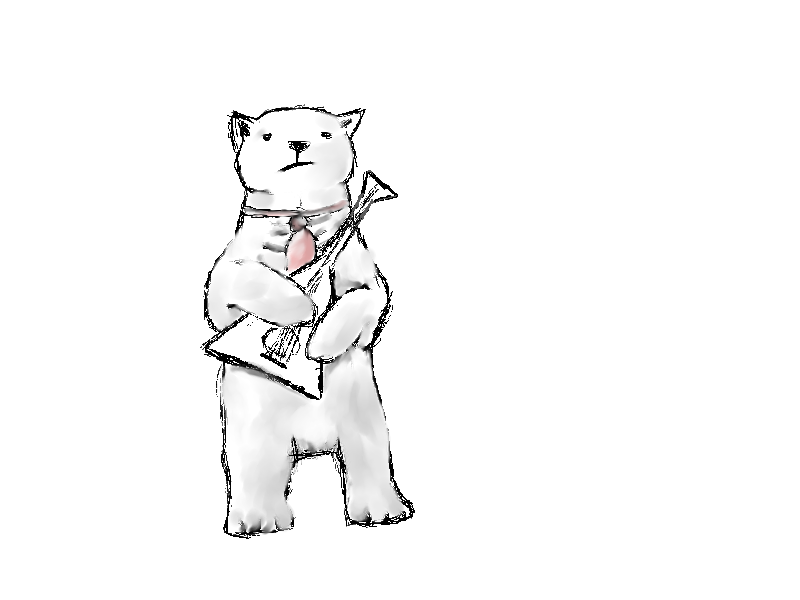
\includegraphics[scale=0.5]{example.png}
            \centering
            \caption{Example Figure}
            \label{fig:example01}
        \end{figure}
        % Figure ----------------------------------------------------------
        
        
    \chapter{Results}
        \section{Performance}
            Performance and memory testing.
        \section{Accuracy}
            Test predictions. MSE, MRSE, etc..
        \section{Possible Improvements}
            Implementation tricks, algorithmic improvement.  
% Main Body ---------------------------------------------------------------

% List of figures
    \listoffigures
% List of figures

% Bibliography ------------------------------------------------------------
    \chapter{Literature}
        \printbibliography
        %\bibliographystyle{unsrt}
        %\bibliography{library}
% Bibliography ------------------------------------------------------------

\end{document}
